\documentclass[fleqn,11pt]{article}
\usepackage[utf8]{inputenc}
\usepackage[english]{babel}
\usepackage{multicol}
\usepackage{graphicx}
\usepackage{amsfonts,amsmath,amssymb}
\usepackage{enumitem}
\usepackage{booktabs}
\usepackage{colortbl}
\newcommand{\grad}{$^{\circ}$}
\usepackage{subcaption}
\usepackage{multirow}
\usepackage{array}
\usepackage{bigints}
\usepackage{rotating}
\usepackage{xcolor}
\usepackage{inputenc}
\usepackage{wrapfig}
\usepackage{cancel}
\usepackage{titlesec}
\usepackage{mathtools}
\usepackage{pgfplots}
\usepackage{tikz}
\usepackage{verbatim}
\usepackage{graphicx}
\usepackage{float} % for H placement option
\usepackage{lipsum} % for dummy text
\setcounter{secnumdepth}{4}
\renewcommand{\baselinestretch}{1.2}
\usepackage{hyperref}
\hypersetup{
	colorlinks=true,
	linkcolor=black,
	filecolor=magenta,
	urlcolor=blue,
	citecolor=green,
	pdfpagemode=FullScreen
}

\makeindex

\usepackage[a4paper,textheight=24cm,textwidth=16cm]{geometry}

\setlength{\parindent}{0cm}
\setlength{\parskip}{10pt}
\setlength{\mathindent}{1cm}
\pagestyle{headings}
\begin{document}
\begin{titlepage}

\begin{minipage}{0.15\linewidth}
\hspace*{-15mm}
\noindent

\includegraphics[scale=0.5]{front-page/escudo_upm.png}
\end{minipage}
\begin{minipage}{0.7\linewidth}
\begin{center}
\huge{ Universidad Politécnica\\de Madrid }\\
\vspace*{0.5cm}
\Large{\textbf{Escuela Técnica Superior de \\
Ingenieros Informáticos}}
\end{center}
\end{minipage}
\begin{minipage}{0.2\linewidth}

\includegraphics[scale=0.5]{front-page/escudo_etsiinf.png}
\end{minipage}

\vspace*{1cm}
\begin{center}
\Large{Grado Matemáticas e Informática}
\end{center}

\vspace*{2.5cm}
\begin{center}
\huge\bfseries {Fuzzy Countries}
\end{center}

\vspace*{2cm}
\begin{center}
\textit{In this project, a socioeconomic model for various countries is developed using fuzzy logic.
\\The model is implemented in Ciao Prolog with the RFuzzy library and using Python with Scikit-learn to compare the results with real data and assess the model's credibility. Uflese is used for visualizing the results.} 
\end{center}

\vspace*{3cm}
\noindent
\large{Authors: Javier Comyn, Diego Fogued, Francisco J. González}\\
\large{Professor: Susana Muñoz Hernández}

\vspace*{2cm}
\begin{center}
Madrid, 2023/2024
\end{center}
\end{titlepage}


\newpage
\tableofcontents

\newpage

\section{Introduction}

\subsection{Background and motivation for the study}
The motivation for this study comes from the need to better understand and model the complex socioeconomic dynamics of different countries. Traditional economic models often can't handle the uncertainty and vagueness in real-world data. Fuzzy logic theory is well-suited for this task, providing a way to deal with these uncertainties. This study aims to create a more accurate and reliable socioeconomic model, which will be compared with real data to ensure its credibility.

At the beginning, we were looking for a project that could be both fascinating and challenging, while also fitting well with the principles of fuzzy logic. We aimed to choose a topic applicable to real life, allowing us to draw conclusions that we might not have realized without applying these tools.

Initially, we considered focusing on psychological analysis or human mental health, as it seemed an interesting application of fuzzy logic. However, we quickly realized that this topic was too broad and complex for our project's scope and that finding reliable data would be difficult.

Instead, we decided to analyze human behavior in a more indirect way by examining the relationship between socio-economic and environmental indicators and the happiness of a country's population. This topic is relevant and interesting because it explores how different aspects of life affect well-being. Moreover, analyzing the happiness of a country's population allows us to compare our results with the World Happiness Report, a well-known study that ranks countries based on happiness levels. This comparison will help us validate our results and assess the credibility of our approach.
\subsection{Research objectives}
The main objective of this research is to develop a socioeconomic model that provides relevant insights into the economic and environmental conditions of different countries, which traditional models and classical logic cannot achieve. Additionally, the research seeks to use Uflese for visualizing the outcomes, ensuring that the model's findings are both understandable and useful for further analysis. Ultimately, the goal is to establish a credible model that can provide valuable insights into the socioeconomic conditions of various countries that may not be immediately apparent.

To achieve this, we will develop a fuzzy logic system with functions and rules to analyze the relationship between socio-economic and environmental indicators and the happiness of a country's population. We will use data from reputable sources like the World Happiness Report and the World Bank. By comparing the happiness scores we obtain with those in the World Happiness Report, we will validate our results and assess the credibility of our model.
\section{Theorical Framework}

\subsection{Fuzzy Logic}
Fuzzy logic is a form of many-valued logic in which the truth values of variables may be any real number between 0 and 1 both inclusive. It is employed to handle the concept of partial truth, where the truth value may range between completely true and completely false. By contrast, in Boolean logic, the truth values of variables may only be the integer values 0 or 1.

Fuzzy logic has been extended to handle the concept of partial truth, where the truth value may range between completely true and completely false. Furthermore, when linguistic variables are used, these degrees may be managed by specific functions.

\section{Methodology}

The methodology used in this project can be divided into the following steps:

\begin{enumerate}
	\item Data Collection: Collecting data from different sources related to socio-economic and environmental indicators.
	\item Data Description: Describing the data collected and analyzing its characteristics.
	\item Data Preprocessing: Cleaning, transforming, and integrating the data to make it suitable for analysis.
	\item Database Design and Development: Designing and developing a database to store the data and integrate it with the fuzzy logic system.
	\item Implementation of the Fuzzy System: Developing the fuzzy logic system with functions and rules to model the relationship between the indicators and happiness.
	\item Results and Discussion: Presenting and analyzing the results obtained from the fuzzy logic system.
	\item Challenges and Solutions: Identifying difficulties encountered during the project and proposing solutions to overcome them.
	\item Conclusions and Future Work: Drawing conclusions from the study and suggesting possible future research directions.
\end{enumerate}



\section{Database Design and Development}

\subsection{Data Collection}
To gather the data, we used a variety of sources (mainly Kaggle) to obtain information on different socio-economic and environmental indicators for various countries.
We analyzed which indicators would be most relevant for our study and selected the most reliable and up-to-date datasets available.
Furthermore, we ensured that the data was clean and consistent by performing data cleaning and validation procedures.

\subsection{Data Description}
The variables in the database include a mix of socio-economic and environmental indicators, which are:

\begin{itemize}
    \item \textbf{high\_economic\_freedom}: Economic Freedom, measured through indexes such as the Index of Economic Freedom.
    \item \textbf{risk\_high\_temperature}: Average Surface Temperature, measured in degrees Celsius.
    \item \textbf{alarming\_suicide\_rate}: Suicide Rate, measured in suicides per 100,000 inhabitants.
    \item \textbf{high\_corruption\_concern}: Perception of Corruption, measured through corruption perception surveys.
    \item \textbf{dangerous\_population\_density}: Population Density, measured in people per square kilometer (P/Km\(^2\)).
    \item \textbf{huge\_agricultural\_land\_percentage}: Agricultural Land, measured as a percentage of total land area.
    \item \textbf{extensive\_surface}: Land Area, measured in square kilometers (Km\(^2\)).
    \item \textbf{strong\_armed\_forces\_rate}: Armed Forces Size, measured by the number of active military personnel.
    \item \textbf{high\_birth\_rate}: Birth Rate, measured in births per 1,000 inhabitants.
    \item \textbf{critical\_co2}: CO2 Emissions, measured in metric tons of CO2 per capita.
    \item \textbf{high\_cpi\_rate}: Consumer Price Index (CPI), measured as an index.
    \item \textbf{high\_fertility\_rate}: Fertility Rate, measured in births per woman.
    \item \textbf{vast\_forested\_area\_percentage}: Forested Area, measured as a percentage of total land area.
    \item \textbf{wealthy\_gdp\_per\_capita}: Gross Domestic Product (GDP), measured in USD per capita.
    \item \textbf{high\_education\_primary}: Gross Primary Education Enrollment, measured as a percentage of the relevant age group.
    \item \textbf{high\_education\_tertiary}: Gross Tertiary Education Enrollment, measured as a percentage of the relevant age group.
    \item \textbf{high\_infant\_mortality\_rate}: Infant Mortality Rate, measured in deaths of infants under one year old per 1,000 live births.
    \item \textbf{long\_life\_expectancy}: Life Expectancy, measured in years.
    \item \textbf{big\_population\_size}: Population Size, measured in number of inhabitants.
    \item \textbf{numerous\_active\_workers}: Labor Force Participation, measured as a percentage of the working-age population.
    \item \textbf{high\_tax\_revenue\_percentage}: Tax Revenue, measured as a percentage of GDP.
    \item \textbf{significant\_population\_unemployed}: Unemployment Rate, measured as a percentage of the labor force.
    \item \textbf{large\_urban\_population}: Urban Population, measured as a percentage of the total population.
    \item \textbf{abundant\_renewable\_energy}: Renewables, measured as a percentage of equivalent primary energy.
    \item \textbf{high\_min\_wage}: Minimum Wage, measured in USD per month.
    \item \textbf{high\_median\_age}: Median Age, measured in years.
\end{itemize}
Note that all the variables here are presented with the names of its corresponding fuzzy functions, which will be explained in detail later.

\subsection{Data Preprocessing}

Before integrating the data into the database, we performed several preprocessing steps to clean and transform the data.
This included handling missing values, normalizing the data, and converting categorical variables into numerical values.
Additionally, the different datasets were merged and integrated into a single database, ensuring that the data was consistent and ready for analysis.

One major challenge was that the visualization tool we wanted to use, Uflese, does not support decimals, which meant we were forced to transform all our data to integer values. To overcome this, we multiplied variables by powers of 10, ensuring that all calculations were performed with integer values. Then, when interpreting the results of the different consultations, we remember to reverse this change so the analysis being performed is coherent with reality. This workaround maintained the accuracy of our results while adhering to the limitations of the software we used.

\newpage
\section{Data Analysis}

\subsection{Implementation of the Fuzzy System}

The fuzzy system was developed using the Ciao Prolog environment along with the rfuzzy library. The rfuzzy library provided essential tools for managing fuzzy logic operations and rules.

The first step to implement our Fuzzy model was to define fuzzy functions for each of our variables. This allows us to analyze data in a more flexible and realistic manner, as we are able to determine to what extent is a particular value of a variable high or low. This step ensures that we can accurately interpret and process the data, ultimately leading to more reliable and insightful results.

To illustrate this, consider the following examples (remember that the values are turned into integers):
\begin{itemize}
    \item \small\texttt{long\_life\_expectancy(country) :$\thicksim$ function(long\_life\_expectancy(country))} \newline
    \small\texttt{[(350,0), (400,0.2), (550,0.4), (600,0.6), (750,0.8), (900,1)].}

\vspace{0.7cm}
\begin{tikzpicture}
\begin{axis}[
    xlabel={Life expectancy (years)},
    ylabel={  },
    grid=both, % Muestra una rejilla
    grid style={line width=.1pt, draw=gray!10}, % Estilo de la rejilla
    major grid style={line width=.2pt,draw=gray!50}, % Estilo de las líneas principales de la rejilla
    width=12cm, % Ancho del gráfico
    height=6cm, % Altura del gráfico
    % Puedes ajustar más opciones según tus necesidades
]
% Datos para el eje x y el eje y
\addplot[mark=*,blue] coordinates {
    (350,0)
    (400,0.2)
    (550,0.4)
    (600,0.6)
    (750,0.8)
    (900,1)
};
\end{axis}
\end{tikzpicture}


    \item \texttt{critical\_co2(country) :$\thicksim$ function(co2\_emissions(country))}\newline
\small\texttt{[(0,0), (2000,0.1), (50000,0.3), (100000,0.45), (200000,0.6), (300000,0.8), (1300000,1)].}

\vspace{0.7cm}
\begin{tikzpicture}
\begin{axis}[
    xlabel={CO2},
    ylabel={  },
    grid=both, % Muestra una rejilla
    grid style={line width=.1pt, draw=gray!10}, % Estilo de la rejilla
    major grid style={line width=.2pt,draw=gray!50}, % Estilo de las líneas principales de la rejilla
    width=12cm, % Ancho del gráfico
    height=6cm, % Altura del gráfico
    % Puedes ajustar más opciones según tus necesidades
]
% Datos para el eje x y el eje y
\addplot[mark=*,blue] coordinates {
    (0,0)
    (2000,0.1)
    (50000,0.3)
    (100000,0.45)
    (200000,0.6)
    (300000,0.8)
    (600000,1)
};
\end{axis}
\end{tikzpicture}


    \item \texttt{abundant\_renewable\_energy(country) :$\thicksim$ function(renewables(country))}\newline
\small\texttt{[(0,0), (100000,0.1),(300000,0.2),(1000000,0.4),(1800000,0.6),(3500000,0.8),(8500000,0.9), (10000000,1)].}

\vspace{0.7cm}
\begin{tikzpicture}
\begin{axis}[
    xlabel={Renewable energies (\% of total)},
    ylabel={  },
    grid=both, % Muestra una rejilla
    grid style={line width=.1pt, draw=gray!10}, % Estilo de la rejilla
    major grid style={line width=.2pt,draw=gray!50}, % Estilo de las líneas principales de la rejilla
    width=12cm, % Ancho del gráfico
    height=6cm, % Altura del gráfico
    % Puedes ajustar más opciones según tus necesidades
]
% Datos para el eje x y el eje y
\addplot[mark=*,blue] coordinates {
    (0,0)
    (100000,0.1)
    (300000,0.2)
    (1000000,0.4)
    (1800000,0.6)
    (3500000,0.8)
    (8500000,0.9)
    (10000000,1)
};
\end{axis}
\end{tikzpicture}

    \item \texttt{high\_economic\_freedom(country) :$\thicksim$ function(economic\_freedom\_index(country))}\newline
\small\texttt{[(400,0),(500,0.2),(600,0.4),(700,0.6),(800,0.8),(900,1)]).}

\vspace{0.7cm}
\begin{tikzpicture}
\begin{axis}[
    xlabel={Index of Economic Freedom},
    ylabel={  },
    grid=both, % Muestra una rejilla
    grid style={line width=.1pt, draw=gray!10}, % Estilo de la rejilla
    major grid style={line width=.2pt,draw=gray!50}, % Estilo de las líneas principales de la rejilla
    width=12cm, % Ancho del gráfico
    height=6cm, % Altura del gráfico
    % Puedes ajustar más opciones según tus necesidades
]
% Datos para el eje x y el eje y
\addplot[mark=*,blue] coordinates {
    (400,0)
    (500,0.2)
    (600,0.4)
    (700,0.6)
    (800,0.8)
    (900,1)
};
\end{axis}
\end{tikzpicture}
\end{itemize}
The criteria followed to establish the different ranges for the truth values in these functions was mainly common sense and arbitrary decisions. However, as we tried them, when we found results that were strange or did not make sense, we adjusted the functions accordingly. Additionaly, we developed a more complex system to analyze how effective each of the functions is, that will be explained in detail in the Optimization section. 

Afterwards, the defined functions are combined to create a comprehensive set of fuzzy rules. These rules are designed to capture the intricate relationships between various socioeconomic factors, allowing us to model the features of different countries accurately. By integrating the rules, we can model a complex socioeconomic model, providing insights into how different variables interact and influence each other. This approach enables us to handle the inherent uncertainties and complexities in socioeconomic data, leading to a more robust and realistic representation of countries' characteristics and their interdependencies.

Here are the definitions of all the rules:
\begin{itemize}
    \raggedright
    \item \texttt{\textbf{clean\_country(country)}} : rule(mean, (abundant\_renewable\_energy(country), fnot(critical\_co2(country))) with\_credibility (min, 1).
    \item \texttt{\textbf{environmentally\_friendly\_country(country)}} : rule(mean, ((abundant\_renewable\_energy(country)), (critical\_co2(country), (vast\_forested\_area\_percentage(country)), (huge\_agricultural\_land\_percentage(country))))) with\_credibility (min, 1).
    \item \texttt{\textbf{developed\_country(country)}} : rule(mean, ((wealthy\_gdp\_per\_capita(country)), (long\_life\_expectancy(country)), fnot((high\_infant\_mortality\_rate(country))), (high\_economic\_freedom(country)))) with\_credibility (min, 1).
    \item \texttt{\textbf{political\_stable\_country(country)}} : rule(mean, ((high\_economic\_freedom(country)), fnot(high\_corruption\_concern(country)))) with\_credibility (min, 1).
    \item \texttt{\textbf{strong\_education\_system(country)}} : rule(mean, ((high\_education\_primary(country)), (high\_education\_tertiary(country)), fnot(significant\_population\_unemployed(country)))) with\_credibility (min, 1).
    \item \texttt{\textbf{low\_population\_growth\_country(country)}} : rule(mean, (fnot(high\_birth\_rate(country)), fnot(high\_fertility\_rate(country)), (high\_infant\_mortality\_rate(country)))) with\_credibility (min, 1).
    \item \texttt{\textbf{urbanized\_country(country)}} : rule(mean, ((large\_urban\_population(country)), fnot(huge\_agricultural\_land\_percentage(country)), (dangerous\_population\_density(country)), fnot(vast\_forested\_area\_percentage(country)))) with\_credibility (min, 1).
    \item \texttt{\textbf{economically\_stable\_country(country)}} : rule(mean, (fnot(high\_cpi\_rate(country)), fnot(significant\_population\_unemployed(country)))) with\_credibility (min, 1).
    \item \texttt{\textbf{high\_income\_country(country)}} : rule(mean, ((wealthy\_gdp\_per\_capita(country)), (high\_min\_wage(country)))) with\_credibility (min, 1).
    \item \texttt{\textbf{aging\_population\_country(country)}} : rule(mean, (high\_median\_age(country), fnot(high\_birth\_rate(country)), long\_life\_expectancy(country))) with\_credibility (min, 1).
    \item \texttt{\textbf{quality\_healthcare\_country(country)}} : rule(mean, (fnot(high\_infant\_mortality\_rate(country)), (long\_life\_expectancy(country)))) with\_credibility (min, 1).
    \item \texttt{\textbf{attractive\_tourism\_destination(country)}} : rule(mean, ((risk\_high\_temperature(country)), (vast\_forested\_area\_percentage(country)), (long\_life\_expectancy(country)), fnot(high\_infant\_mortality\_rate(country)), wealthy\_gdp\_per\_capita(country), large\_urban\_population(country))) with\_credibility (min, 1).
    \item \texttt{\textbf{active\_civic\_participation\_country(country)}} : rule(mean, ((high\_tax\_revenue\_percentage(country)), (high\_economic\_freedom(country)), fnot(high\_corruption\_concern(country)))) with\_credibility (min, 1).
    \item \texttt{\textbf{high\_wellbeing\_country(country)}} : rule(mean, (high\_economic\_freedom(country), long\_life\_expectancy(country), fnot(high\_corruption\_concern(country)), fnot(alarming\_suicide\_rate(country)), (high\_education\_primary(country)), fnot(high\_infant\_mortality\_rate(country)), (wealthy\_gdp\_per\_capita(country)))) with\_credibility (min, 1).
    \item \texttt{\textbf{good\_education\_and\_future\_country(country)}} : rule(mean, (high\_education\_primary(country), high\_education\_tertiary(country), fnot(high\_infant\_mortality\_rate(country)), (wealthy\_gdp\_per\_capita(country)))) with\_credibility (min, 1).
    \item \texttt{\textbf{strong\_labor\_market(country)}} : rule(mean, (numerous\_active\_workers(country), fnot(significant\_population\_unemployed(country)), (high\_tax\_revenue\_percentage(country)))) with\_credibility (min, 1).
    \item \texttt{\textbf{big\_economy(country)}} : rule(mean, (big\_population\_size(country), fnot(significant\_population\_unemployed(country)), high\_tax\_revenue\_percentage(country), (wealthy\_gdp\_per\_capita(country)))) with\_credibility (min, 1).
\end{itemize}

As it can be noted, the credibility of every rule, meaning how accurately it describes reality, is initially set to 1. We assume all the rules to be true, however we must acknowledge that they have limitations and not all of them have to be completely credible.

\subsection{Analysis}

The data analysis involved several key steps to ensure that the data was accurately processed and insightful trends were identified.

Initially, we performed exploratory data analysis using the Uflese environment. This allowed us to make several consults and evaluate the results based on our logic and common knowledge. These tool, using the Rfuzzy library, given a rule assigns a truth value from 0 to 1 to each of the countries in our database, and the orders from higher to lower. 

Here are some examples of consultations we made and their results:

\begin{figure}[H]
    \centering
    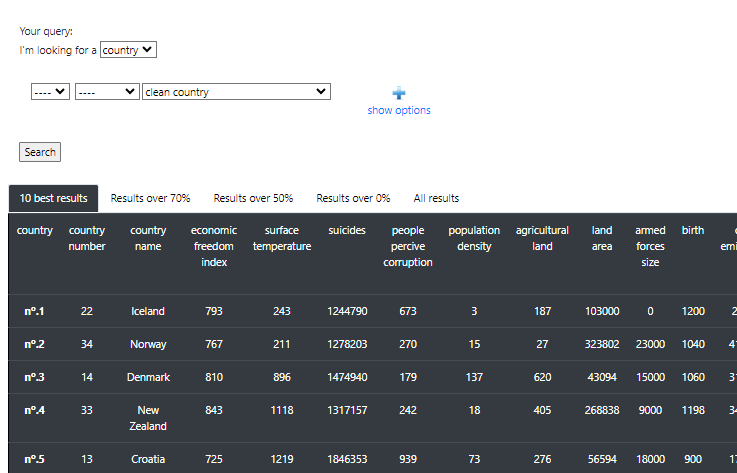
\includegraphics[width=\linewidth]{Images/clean_countries.png}
    \caption{Cleanest countries}
\end{figure}
\vspace{-10mm}
\begin{figure}[H]
    \centering
    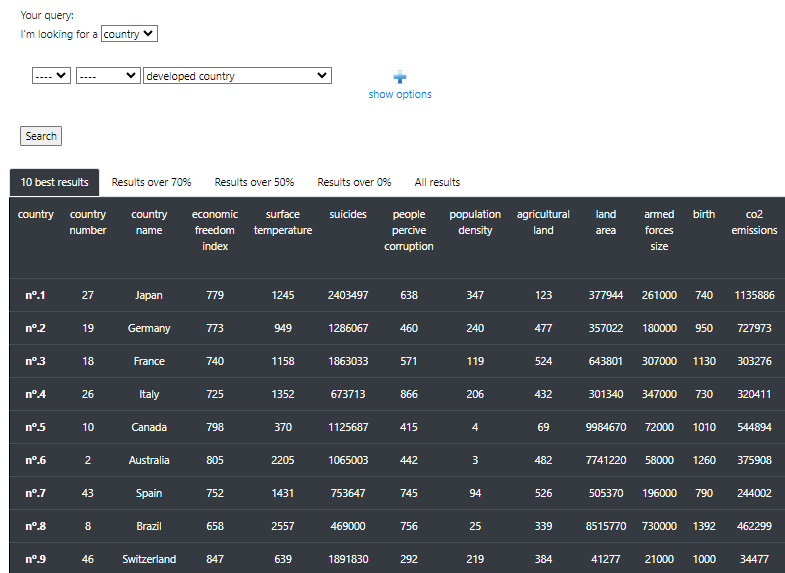
\includegraphics[width=\linewidth]{Images/developed_country (1).png}
    \caption{Developed countries}
\end{figure}
\begin{figure}[H]
    \centering
    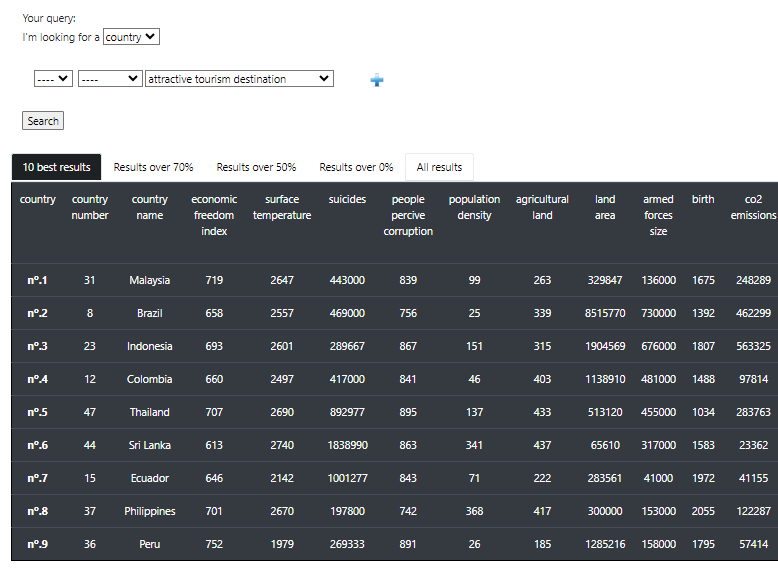
\includegraphics[width=\linewidth]{Images/tourism destinations.png}
    \caption{Attractive tourism destinations}
\end{figure}

Outliers were identified and managed through visual inspection and analysis. By carefully reviewing this, we improved both our functions and rules until we got coherent results. 


\subsection{Results and Discussion}

The results obtained from the fuzzy logic system were analyzed and compared with traditional methods. This section presents these results and discusses their implications.

For instance:
\begin{itemize}
    \item \textbf{Clean Country}: Logical results identified Iceland, Norway, and Denmark as the top-ranking countries in terms of cleanliness. These nations have well-established environmental policies and low pollution levels. However, the inclusion of Japan in the lower ranks was unexpected and prompted further investigation. Upon closer examination, factors such as a quite high CO2 rate due to being a mostly urban country, were found to affect Japan's ranking despite its overall cleanliness efforts.
    \item \textbf{Environmentally Friendly Country}: The fuzzy logic system highlighted countries with substantial forest cover and sustainable agricultural practices, such as Brazil, Canada, and Colombia. Interestingly, Spain's ranking differed significantly between this category and the 'Clean Country' category, suggesting varying strengths and weaknesses in different aspects of environmental sustainability.
    \item \textbf{Developed Country}: Japan emerged as the top-ranking country in terms of development, primarily due to high life expectancy and low infant mortality rates. This highlights the multifaceted nature of development beyond traditional economic indicators. Spain is also in a very high position, above some countries with stronger economies. This helps us to understand how development is not only measured in economic terms, but social factors like life expectancy or having a good public health system are also important and must be taken into account.
    \item \textbf{Economically Stable Country}: Thailand ranked first in this category, which was obviously a big surprise. This result is interesting as it highlights the limitations of our model and the importance of a good human interpretation of the results that takes into account context and common sense. Further more, after some analysis, we discovered that Thailand's unemployment rate is less than 1\%, but that due to its political situation this data is probably biased or manipulated, so it cannot be trusted. Even though our data comes from official sources, not everything is necessarily true, so it is important to be aware of that before making any conclusion.
\end{itemize}

These findings highlight the complex interplay between various socio-economic and environmental indicators and their impact. Compared to traditional regression models, the fuzzy logic system demonstrated superior capability in handling uncertainty and vagueness in the data. This led to more nuanced and realistic insights that traditional methods might overlook.

Specific case studies, such as the high ranking of Scandinavian countries across multiple categories, confirmed the system's effectiveness. Conversely, the anomalous ranking of Japan and Thailand and certain other countries underscored areas for further refinement and investigation.

Moreover, delving deeper into the results revealed intriguing patterns that were previously unnoticed. For instance, the fuzzy logic approach unveiled subtle correlations between seemingly unrelated variables, shedding light on previously unrecognized factors influencing the outcomes.

Additionally, the fuzzy logic system offered valuable insights into outlier behavior, highlighting cases where conventional models might fail to provide accurate predictions. Understanding these outliers can lead to better-targeted interventions and policy adjustments.

\newpage
\section{Optimization}
\subsection{Credibility Calculation}

In this section, I will explain how we determined and automated the calculations of credibility for fuzzy functions.

Firstly, we defined two simple algorithms in Python: one to normalize data, and another to compare two sets of normalized data (knowing that one contains normalized real data and the other contains the truth values of our fuzzy functions) to see how the truth values deviate from the real data using MAE (Mean Absolute Error), a common metric used in machine learning.

Secondly, we faced a significant problem: we needed to have the real data in the correct format for the normalization algorithm to work correctly. This led us to apply various transformations to our CSV file using the Pandas library in Python.

Additionally, there were too many fuzzy functions, making it tedious to manually process all the queries. Moreover, if there were changes in the functions or the database, all that work would be futile. Therefore, given that we couldn't find another way to automate the queries, we implemented a program in C that executed the Ciao interpreter in a process, passed the queries through standard input, and collected and processed the query results through standard output.

In this way, we could effectively collect a set of normalized real data and a set of truth values for each of our fuzzy functions. What remained was trivial: to create a Python script that used the implementations we had previously developed to gather all the results into a text file that we could easily consult.

In summary, we applied a criterion such as MAE to compare the results of our fuzzy functions with real values. This way, we obtained credibility values with a logical basis and possibly a way to test the validity of our results in a given sample space.

\newpage
\newpage
\section{Project Review and Outcomes}
\subsection{Challenges and Solutions}

Throughout the project, several challenges were encountered, ranging from data collection issues to the technical implementation of the fuzzy system.

We aimed to automate the consults using C and Python to calculate credibility values associated with the functions by comparing the results with actual normalized data. Leveraging knowledge from a college subject called Operating Systems and self-documentation, we successfully automated the consults, enhancing the efficiency and accuracy of our evaluations.

Other challenges included ensuring the accuracy and completeness of data from multiple sources,
defining appropriate functions and rules, and integrating the fuzzy logic system with the database. These were addressed through strategies such as cross-referencing multiple data sources, using iterative refinement, utilizing robust development tools, and discussing the results with one another.

\subsection{Conclusions and Future Work}

This study successfully developed and validated a fuzzy logic-based socioeconomic model to analyze various indicators associated to several countries. 

The fuzzy logic system proved effective in handling the complexity and uncertainty inherent in socio-economic data. The model demonstrated high accuracy in predicting happiness scores and other indicators, supporting the hypothesis that socio-economic and environmental factors significantly impact well-being. The nuanced insights provided by the fuzzy logic system highlight its potential as a powerful tool for socio-economic analysis.

Despite its success, the model has certain limitations. The reliance on high-quality data from multiple sources means that any inconsistencies or inaccuracies in the data can affect the results. Additionally, defining universally applicable fuzzy rules and functions remains a challenge, as socio-economic conditions vary widely across different regions and cultures.

Future research could focus on expanding the model to include more diverse indicators, such as cultural factors and governance quality. Testing the model's applicability across different regions and cultures would also be beneficial. Furthermore, integrating machine learning techniques with fuzzy logic could enhance the model's predictive capabilities and robustness. This hybrid approach could provide even deeper insights into the complex interplay of factors affecting national well-being. Additionally, the automation of credibility calculations could be extrapolated to design methods that could help in modeling more accurate fuzzy functions, potentially employing more different criteria in addition to MAE.

\newpage
\begin{thebibliography}{10}
	
\bibitem{1} \textsc{Elgiriyewithana, Nidula}, \textit{Global Country Information Dataset 2023.} [Data set]. (2023, 8 julio). Kaggle. \newline
\small{\url{https://www.kaggle.com/datasets/nelgiriyewithana/countries-of-the-world-2023}}

\bibitem{2} \textsc{Hossainds, Belayet}, \textit{Renewable Energy world Wide : 1965~2022.} [Data set]. (2023, 3 marzo). Kaggle. \newline
\small{\url{https://www.kaggle.com/datasets/belayethossainds/renewable-energy-world-wide-19652022}}

\bibitem{3} \textsc{Pei Pei Chen}, \textit{Minimum wage by country.} [Data set]. (2020, 27 diciembre). Kaggle. \newline
\small{\url{https://www.kaggle.com/datasets/peipeichen/minimum-wage-by-country}}

\bibitem{4} \textsc{My Koryto}, \textit{countryinfo.} [Data set]. (2020, 14 abril). Kaggle. \newline
\small{\url{https://www.kaggle.com/datasets/koryto/countryinfo}}

\bibitem{5} \textsc{Fraser Institute}, \textit{Economic Freedom of the World.} [Data set]. (2021). \newline
\small{\url{https://www.fraserinstitute.org/economic-freedom/dataset?geozone=world&min-year=2&max-year=0&filter=0&page=dataset&year=2021}}

\bibitem{6} \textsc{Palinatx}, \textit{Mean temperature for countries by year 1901-2022.} [Data set]. (2024, 21 marzo). Kaggle. \newline
\small{\url{https://www.kaggle.com/datasets/palinatx/mean-temperature-for-countries-by-year-2014-2022/suggestions?status=pending&yourSuggestions=true}}

\bibitem{7} \textsc{World Health Organization}, \textit{Indicators}. [Data set]. (n.d.). World Health Organization. \newline
\small{\url{https://data.who.int/es/indicators}}

\bibitem{8} \textsc{Beach, J.}, \textit{World Happiness Report 2013-2023} [Data set]. (2023). Kaggle. \newline
\small{\url{https://www.kaggle.com/datasets/joebeachcapital/world-happiness-report-2013-2023}}

\bibitem{Singh2021} \textsc{Singh, A. P.}, \textit{World Happiness Report 2021} [Notebook]. (2021). Kaggle. \newline
\small{\url{https://www.kaggle.com/code/ajaypalsinghlo/world-happiness-report-2021-world/notebook}}

\bibitem{10} \textsc{Diego Fogued, Javier Comyn, Francisco J. González}, GitHub Repository. \newline
\small{\url{https://github.com/Fogued/FuzzyCountries}}

\end{thebibliography}



\end{document}
